
%{{第六回}}{第六回}}

\chapter{贾宝玉初试云雨情 刘姥姥一进荣国府}

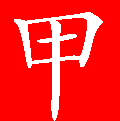
\includegraphics[width=3mm]{../Images/00002}{\kaishu 宝玉、袭人亦大家常事耳,写得是已全领警幻意淫之训。此回借刘妪,却是写阿凤正传,并非泛文,且伏``二进''``三进''及巧姐之归着。

此回刘妪一进荣国府,用周瑞家的,又过下回无痕,是无一笔写一人文字之笔。

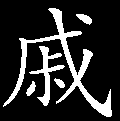
\includegraphics[width=3mm]{../Images/00005}风流真假一般看,借贷亲疏触眼酸。总是幻情无了处,银灯挑尽泪漫漫。}

题曰:

朝叩富儿门,富儿犹未足。虽无千金酬,嗟彼胜骨肉。

却说秦氏因听见宝玉从梦中唤他的乳名,心中自是纳闷,又不好细问。彼时宝玉迷迷惑惑,若有所失。众人忙端上桂圆汤来,呷了两口,遂起身整衣。袭人伸手与他系裤带时,不觉伸手至大腿处,只觉冰凉一片粘湿。唬的忙退出手来,问是怎么了。宝玉红涨了脸,把他手一捻。袭人本是个聪明女子,年纪本又比宝玉大两岁,近来也渐通人事,今见宝玉如此光景,心中便觉察了一半,不觉也羞的红涨了脸面,{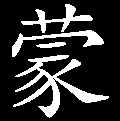
\includegraphics[width=3mm]{../Images/00006}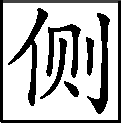
\includegraphics[width=3mm]{../Images/00011}\footnotesize \kaishu 存身分。}遂不敢再问。{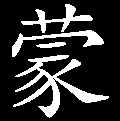
\includegraphics[width=3mm]{../Images/00006}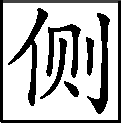
\includegraphics[width=3mm]{../Images/00011}\footnotesize \kaishu 既少通人事,无心者则再不复问矣;既问,则无限幽思,皆在于伏身之一笑,所以必当有偷试之一番。行文轻巧,皆出于自然,毫无一些勉强。妙极!}仍旧理好衣裳,遂至贾母处来,胡乱吃毕晚饭,过这边来。

袭人忙趁众奶娘丫鬟不在旁时,另取出一件中衣来与宝玉换上。宝玉含羞央告道:``好姐姐,千万别告诉别人,要紧!''袭人亦含羞笑问道:``你梦见什么故事了?{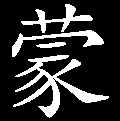
\includegraphics[width=3mm]{../Images/00006}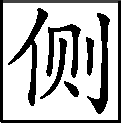
\includegraphics[width=3mm]{../Images/00011}\footnotesize \kaishu 是必当问者。若不问则下文涉于唐突。}是那里流出来的些脏东西?''宝玉道:``一言难尽。''说着,便把梦中之事细说与袭人听了,然后说至警幻所授云雨之情,羞的袭人掩面伏身而笑。{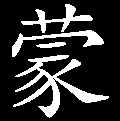
\includegraphics[width=3mm]{../Images/00006}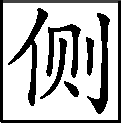
\includegraphics[width=3mm]{../Images/00011}\footnotesize \kaishu 试想。}宝玉亦素喜袭人柔媚姣俏,遂强袭人同领警幻所训云雨之事。{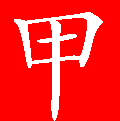
\includegraphics[width=3mm]{../Images/00002}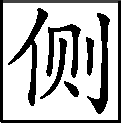
\includegraphics[width=3mm]{../Images/00011}\footnotesize \kaishu 数句文完一回提纲文字。}袭人素知贾母已将自己与了宝玉的,今便如此,亦不为越礼,{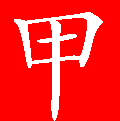
\includegraphics[width=3mm]{../Images/00002}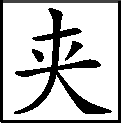
\includegraphics[width=3mm]{../Images/00012}\footnotesize \kaishu 写出袭人身份。}遂和宝玉偷试一番,幸得无人撞见。自此宝玉视袭人更与别个不同,{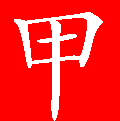
\includegraphics[width=3mm]{../Images/00002}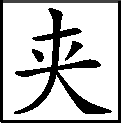
\includegraphics[width=3mm]{../Images/00012}\footnotesize \kaishu 伏下晴雯。}袭人侍宝玉更为尽职。{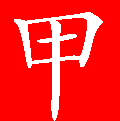
\includegraphics[width=3mm]{../Images/00002}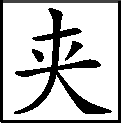
\includegraphics[width=3mm]{../Images/00012}\footnotesize \kaishu 一段小儿女之态,可谓追魂摄魄之笔。}暂且别无话说。{{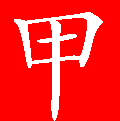
\includegraphics[width=3mm]{../Images/00002}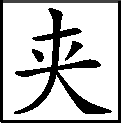
\includegraphics[width=3mm]{../Images/00012}\footnotesize \kaishu 一句{(接)}{[}结{]}住上回``红楼梦''大篇文字,另起本回正文。}}

按荣府中一宅中合算起来,人口虽不多,从上至下也有三四百丁;事虽不多,一天也有一二十件,竟如乱麻一般,并没个头绪可作纲领。正寻思从那一件事、自那一个人写起方妙,恰好忽从千里之外、芥豆之微、小小一个人家,因与荣府略有些瓜葛,{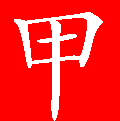
\includegraphics[width=3mm]{../Images/00002}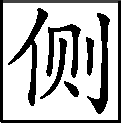
\includegraphics[width=3mm]{../Images/00011}\footnotesize \kaishu ``略有些瓜葛'',是数十回后之正脉也。真千里伏线。}这日正往荣府中来,因此便就此一家说来,倒还是头绪。你道这一家姓甚名谁,又与荣府有甚瓜葛?诸公若嫌琐碎粗鄙呢,则快掷下此书,另觅好书去醒目;{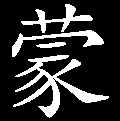
\includegraphics[width=3mm]{../Images/00006}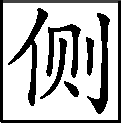
\includegraphics[width=3mm]{../Images/00011}\footnotesize \kaishu {(加)}{[}夹{]}杂世态,巧伏下文。}若谓聊可破闷时,待蠢物{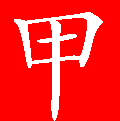
\includegraphics[width=3mm]{../Images/00002}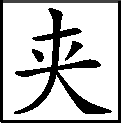
\includegraphics[width=3mm]{../Images/00012}\footnotesize \kaishu 妙谦,是石头口角。}逐细言来。

方才所说的这小小一家,乃本地人氏,姓王,祖上曾作过小小的一个京官,昔年曾与凤姐之祖、王夫人之父识认,因贪王家的势利,便连了宗认作侄儿。{{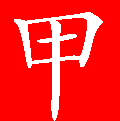
\includegraphics[width=3mm]{../Images/00002}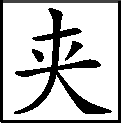
\includegraphics[width=3mm]{../Images/00012}\footnotesize \kaishu 与贾雨村遥遥相对。 }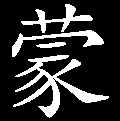
\includegraphics[width=3mm]{../Images/00006}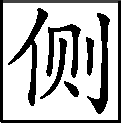
\includegraphics[width=3mm]{../Images/00011}\footnotesize \kaishu 可怜。}那时只有王夫人之大兄、凤姐之父{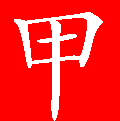
\includegraphics[width=3mm]{../Images/00002}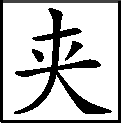
\includegraphics[width=3mm]{../Images/00012}\footnotesize \kaishu 两呼两起,不过欲观者自醒。}与王夫人随在京中的,知有此一门远族,馀者皆不识认。{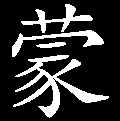
\includegraphics[width=3mm]{../Images/00006}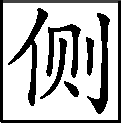
\includegraphics[width=3mm]{../Images/00011}\footnotesize \kaishu 强认亲的榜样。}目今其祖已故,只有一个儿子,名唤王成,因家业萧条,仍搬出城外原乡中住去了。王成新近亦因病故,只有其子,小名狗儿,亦生一子,小名板儿,嫡妻刘氏,又生一女,名唤青儿。{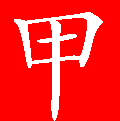
\includegraphics[width=3mm]{../Images/00002}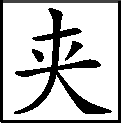
\includegraphics[width=3mm]{../Images/00012}\footnotesize \kaishu 《石头记》中公勋世宦之家以及草莽庸俗之族,无所不有,自能各得其妙。}一家四口,仍以务农为业,因狗儿白日间又作些生计,刘氏又操井臼等事,青板姊妹\href{../Text/part0010_split_000.html\#lnkback_1_a}{\textsuperscript{①}}两个无人看管,狗儿遂将岳母刘姥姥{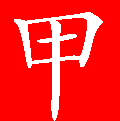
\includegraphics[width=3mm]{../Images/00002}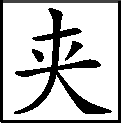
\includegraphics[width=3mm]{../Images/00012}\footnotesize \kaishu 音老,出《谐声字笺》。称呼毕肖。}接来一处过活。{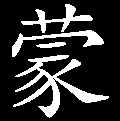
\includegraphics[width=3mm]{../Images/00006}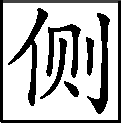
\includegraphics[width=3mm]{../Images/00011}\footnotesize \kaishu 总是用{(过)}{[}逼{]}近法。}这刘姥姥乃是个久经世代的老寡妇,膝下又无儿女,只靠两亩薄田地度日。如今女婿接来养活,岂不愿意,遂一心一计,帮趁着女儿女婿过活起来。

因这年秋尽冬初,天气冷将上来,家中冬事未办,狗儿未免心中烦虑,吃了几杯闷酒,在家闲寻气恼,{{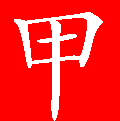
\includegraphics[width=3mm]{../Images/00002}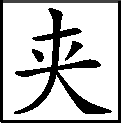
\includegraphics[width=3mm]{../Images/00012}\footnotesize \kaishu 病此病人不少,请来看狗儿。 }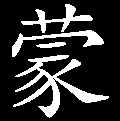
\includegraphics[width=3mm]{../Images/00006}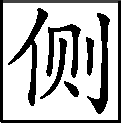
\includegraphics[width=3mm]{../Images/00011}\footnotesize \kaishu 贫苦人多有此等景象。}刘氏不敢顶撞。{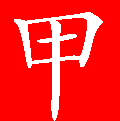
\includegraphics[width=3mm]{../Images/00002}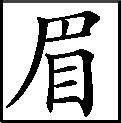
\includegraphics[width=3mm]{../Images/00010}\footnotesize \kaishu 自``红楼梦''一回至此,则珍馐中之虀耳,好看煞!}因此刘姥姥看不过,乃劝道:``姑夫,你别嗔着我多嘴。咱们村庄人,那一个不是老老诚诚的,多大碗吃多大的饭?{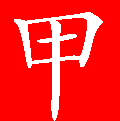
\includegraphics[width=3mm]{../Images/00002}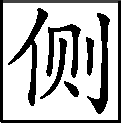
\includegraphics[width=3mm]{../Images/00011}\footnotesize \kaishu 能两亩薄田度日,方说的出来。}你皆因年小时,托着你那老家的福,{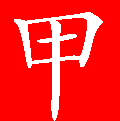
\includegraphics[width=3mm]{../Images/00002}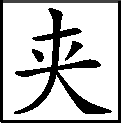
\includegraphics[width=3mm]{../Images/00012}\footnotesize \kaishu 妙称,何肖之至!}吃喝惯了,如今所以把持不住。有了钱就顾头不顾尾,没了钱就瞎生气,成个什么男子汉大丈夫了!{{\includegraphics[width=3mm]{../Images/00002}\includegraphics[width=3mm]{../Images/00012}\footnotesize \kaishu 为纨裤下针,却先从此等小处写来。 \includegraphics[width=3mm]{../Images/00002}\includegraphics[width=3mm]{../Images/00011}\footnotesize \kaishu 此口气自何处得来? }\includegraphics[width=3mm]{../Images/00006}\includegraphics[width=3mm]{../Images/00011}\footnotesize \kaishu 英雄失足,千古同慨。笑煞天下一切。}如今咱们虽离城住着,终是天子脚下。这长安城中,遍地都是钱,只可惜没人会拿去罢了。在家跳蹋也没中用的。''狗儿听说,便急道:``你老只会炕头儿上混说,难道叫我打劫偷去不成?''{\includegraphics[width=3mm]{../Images/00006}\includegraphics[width=3mm]{../Images/00011}\footnotesize \kaishu 古人有错用盗字之说,的是此句章本。}刘姥姥道:``谁叫你偷去呢。到底大家想方法儿裁度,不然,那银子钱自己跑到咱家来不成?''狗儿冷笑道:``有法儿还等到这会子呢!我又没有收税的亲戚,{\includegraphics[width=3mm]{../Images/00002}\includegraphics[width=3mm]{../Images/00012}\footnotesize \kaishu 骂死。}作官的朋友,{\includegraphics[width=3mm]{../Images/00002}\includegraphics[width=3mm]{../Images/00012}\footnotesize \kaishu 骂死。}有什么法子可想的?便有,也只怕他们未必来理我们呢!''

刘姥姥道:``这倒不然。谋事在人,成事在天。咱们谋到了,靠菩萨的保佑,有些机会,也未可知。我倒替你们想出一个机会来。当日你们原是和金陵王家{\includegraphics[width=3mm]{../Images/00002}\includegraphics[width=3mm]{../Images/00012}\footnotesize \kaishu 四字便抵一篇世家传。}连过宗的,二十年前,他们看承你们还好,如今自然是你们拉硬屎,不肯去俯就他,{\includegraphics[width=3mm]{../Images/00006}\includegraphics[width=3mm]{../Images/00011}\footnotesize \kaishu 天下事无有不可为者。总因打不破,若打破时何事不能?请看刘姥姥一篇议论,便应解得些个才是。}故疏远起来。想当初我和女儿还去过一遭。{\includegraphics[width=3mm]{../Images/00002}\includegraphics[width=3mm]{../Images/00012}\footnotesize \kaishu 补前文之未到处。}他家的二小姐着实响快会待人的,倒不拿大。如今现是荣国府贾二老爷的夫人。听得说,如今上了年纪,越发怜贫恤老,最爱斋僧敬道,舍米舍钱的。如今王府虽升了边任,只怕这二姑太太还认得咱们。你何不去走动走动,或者他念旧,有些好处,也未可定。只要他发一点好心,拔一根寒毛比咱们的腰还粗呢!''刘氏一旁接口道:``你老虽说得是,但只你我这样个嘴脸,怎么好到他门上去的?先不先,他们那些门上人也未必肯去通报。没的去打嘴现世。''{\includegraphics[width=3mm]{../Images/00006}\includegraphics[width=3mm]{../Images/00011}\footnotesize \kaishu ``打嘴现世''等字,误尽多少苍生,也能成全多少事体。}

谁知狗儿名利心甚重,{\includegraphics[width=3mm]{../Images/00002}\includegraphics[width=3mm]{../Images/00012}\footnotesize \kaishu 调侃语。}听如此一说,心下便有些活动起来。又听他妻子这番话,便笑接道:``姥姥既如此说,况且当年你又见过这姑太太一次,何不你老人家明日就走一趟,先试试风头再说。''刘姥姥道:``嗳哟哟!{\includegraphics[width=3mm]{../Images/00002}\includegraphics[width=3mm]{../Images/00011}\footnotesize \kaishu 口声如闻。}可是说的,`侯门深似海',我是个什么东西,他家人又不认得我,我去了也是白去的。''狗儿笑道:``不妨,我教你老一个法子:你竟带了外孙子小板儿,先去找陪房周瑞,若见了他,就有些意思了。这周瑞先时曾和我父亲交过一桩事,我们极好的。''{{\includegraphics[width=3mm]{../Images/00002}\includegraphics[width=3mm]{../Images/00012}\footnotesize \kaishu 欲赴豪门,必先交其仆。写来一叹。 }\includegraphics[width=3mm]{../Images/00006}\includegraphics[width=3mm]{../Images/00011}\footnotesize \kaishu 画出当日品行。}刘姥姥道:``我也知道他的。只是许多时不走动,知道他如今是怎么样?这也说不得了,你又是个男人,又这样个嘴脸,自然去不得,我们姑娘年轻媳妇子,也难卖头卖脚去,倒还是舍着我这付老脸去碰一碰。果然有些好处,大家都有益,便是没银子来,我也到那公府侯门见一见世面,也不枉我一生。''说毕,大家笑了一回。当晚计议已定。

次日天未明,刘姥姥便起来梳洗了,又将板儿教训几句。那板儿才亦五六岁的孩子,一无所知,听见带他进城逛\href{../Text/part0010_split_000.html\#lnkback_2_a}{\textsuperscript{②}}{\includegraphics[width=3mm]{../Images/00002}\includegraphics[width=3mm]{../Images/00012}\footnotesize \kaishu 音光,去声。游也。出《谐声字笺》。}去,便喜的无不应承。于是刘姥姥带他进城,找至宁荣街。{\includegraphics[width=3mm]{../Images/00002}\includegraphics[width=3mm]{../Images/00012}\footnotesize \kaishu 街名。本地风光,妙!}来至荣府大门石狮子前,只见簇簇的轿马,刘姥姥便不敢过去,且弹弹衣服,又教了板儿几句话,然后\includegraphics[width=4mm]{../images/00015}{\includegraphics[width=3mm]{../Images/00002}\includegraphics[width=3mm]{../Images/00011}\footnotesize \kaishu ``\includegraphics[width=3mm]{../images/00016}''字神理。}到角门前。只见几个挺胸叠肚、指手画脚的人,坐在大凳上说东谈西呢。{{\includegraphics[width=3mm]{../Images/00002}\includegraphics[width=3mm]{../Images/00012}\footnotesize \kaishu 不知如何想来,又为侯门三等豪奴写照。 }\includegraphics[width=3mm]{../Images/00006}\includegraphics[width=3mm]{../Images/00011}\footnotesize \kaishu 世家奴仆个个皆然,形容逼真。}刘姥姥只得\includegraphics[width=4mm]{../images/00015}上来问:``太爷们纳福。''众人打量了他一会,便问是那里来的。刘姥姥陪笑道:``我找太太的陪房周大爷的,烦那位太爷替我请他出来。''那些人听了,都不瞅睬,半日方说道:``你远远的那墙角下等着,{\includegraphics[width=3mm]{../Images/00006}\includegraphics[width=3mm]{../Images/00011}\footnotesize \kaishu 故套。}一会子他们家有人就出来的。''内中有一年老的说道:``不要误他的事,何苦耍他。''因向刘姥姥道:``那周大爷已往南边去了。他在后一带住着,他娘子却在家。你要找时,从这边绕到后街上后门上问就是了。''{{\includegraphics[width=3mm]{../Images/00002}\includegraphics[width=3mm]{../Images/00012}\footnotesize \kaishu 有年纪人诚厚,亦是自然之理。 }\includegraphics[width=3mm]{../Images/00006}\includegraphics[width=3mm]{../Images/00011}\footnotesize \kaishu 转换法。写门上豪奴不能尽是规矩,故用转换法则不强硬,而笔气自顺。}

刘姥姥听了谢过,遂携了板儿,绕到后门上。只见门前歇着些生意担子,也有卖吃的,也有卖顽意物件的,闹烘烘三二十个孩子在那里厮闹。{\includegraphics[width=3mm]{../Images/00002}\includegraphics[width=3mm]{../Images/00012}\footnotesize \kaishu 如何想来?合眼如见。}刘姥姥便拉住了一个道:``我问哥儿一声,有个周大娘可在家么?''孩子道:``那个周大娘?我们这里周大娘有三个呢,还有两个周奶奶,不知是那一行当上的?''刘姥姥道:``是太太的陪房周瑞。''孩子道:``这个容易,你跟我来。''说着,跳跳蹿蹿的引着刘姥姥进了后门,{\includegraphics[width=3mm]{../Images/00002}\includegraphics[width=3mm]{../Images/00011}\footnotesize \kaishu 因女眷,又是后门,故容易引入。}至一院墙边,指与刘姥姥道:``这就是他家。''又叫道:``周大娘,有个老奶奶来找你呢。''

周瑞家的在内听说,忙迎了出来,问:``是那位?''刘姥姥忙迎上来问道:``好呀,周嫂子!''周瑞家的认了半日,方笑道:``刘姥姥,你好呀!你说说,能几年,我就忘了。{\includegraphics[width=3mm]{../Images/00002}\includegraphics[width=3mm]{../Images/00011}\footnotesize \kaishu 如此口角,从何处出来?}请家里来坐罢。''刘姥姥一壁走,一壁笑说道:``你老是贵人多忘事,那里还记得我们了。''说着,来至房中。周瑞家的命雇的小丫头倒上茶来吃着,周瑞家的又问板儿``长的这么大了'',又问些别后闲语,再问刘姥姥:``今日还是路过,还是特来的?''{{\includegraphics[width=3mm]{../Images/00002}\includegraphics[width=3mm]{../Images/00011}\footnotesize \kaishu 问的有情理。 }\includegraphics[width=3mm]{../Images/00006}\includegraphics[width=3mm]{../Images/00011}\footnotesize \kaishu 刘姥姥此时一团要紧事在心,有问不得不答,递转递进,不敢陟然看之,令人可怜。而大英雄亦有若此者,所谓``欲图大事,不拘小节。''}刘姥姥便说:``原是特来瞧瞧你嫂子,二则也请请姑太太的安。若可以领我见一见更好,若不能,便借重嫂子转致意罢了。''{\includegraphics[width=3mm]{../Images/00002}\includegraphics[width=3mm]{../Images/00012}\footnotesize \kaishu 刘婆亦善于权变应酬矣。}

周瑞家的听了,便猜着几分意思。只因昔年他丈夫周瑞争买田地一事,其中多得狗儿之力,今见刘姥姥如此而来,心中难却其意,{\includegraphics[width=3mm]{../Images/00002}\includegraphics[width=3mm]{../Images/00012}\footnotesize \kaishu 在今世,周瑞妇算是个怀情不忘的正人。}二则也要显弄自己体面。{{\includegraphics[width=3mm]{../Images/00002}\includegraphics[width=3mm]{../Images/00010}\footnotesize \kaishu ``也要显弄''句为后文作地步也。陪房本心本意实事。 }\includegraphics[width=3mm]{../Images/00006}\includegraphics[width=3mm]{../Images/00011}\footnotesize \kaishu 实有此等情理。}听如此说,便笑说:``姥姥你放心,{\includegraphics[width=3mm]{../Images/00002}\includegraphics[width=3mm]{../Images/00011}\footnotesize \kaishu 自是有宠人声口。}大远的诚心诚意的来了,岂有个不教你见个真佛去的?{\includegraphics[width=3mm]{../Images/00002}\includegraphics[width=3mm]{../Images/00012}\footnotesize \kaishu 好口角。}论理,人来客至回话,却不与我们相干。我们这里都是各占一枝儿:{\includegraphics[width=3mm]{../Images/00002}\includegraphics[width=3mm]{../Images/00011}\footnotesize \kaishu 略将荣府中带一带。}我们男的只管春秋两季地租子,闲时只带着小爷们出门就完了,我只管跟太太奶奶们出门的事。皆因你原是太太的亲戚,又拿我当个人,投奔了我来,我竟破个例,给你通个信去。但只一件,姥姥有所不知,我们这里又比不得五年前了。如今太太竟不大管事了,都是琏二奶奶当家。你道这琏二奶奶是谁?就是太太的内侄女,当日大舅爷的女儿,小名凤哥的。''刘姥姥听了,罕问道:``原来是他!怪道呢,我当日就说他不错呢。{\includegraphics[width=3mm]{../Images/00002}\includegraphics[width=3mm]{../Images/00012}\footnotesize \kaishu 我亦说不错。}这等说来,我今儿还得见他了。''周瑞家的道:``这个自然的。如今太太事多心烦,有客来了,略可推得去的也就推过去了,都是这凤姑娘周旋迎待。今儿宁可不见太太,倒要见他一面,{\includegraphics[width=3mm]{../Images/00006}\includegraphics[width=3mm]{../Images/00011}\footnotesize \kaishu {(礼)}{[}理{]}势必然。}才不枉这里来一遭。''刘姥姥道:``阿弥陀佛!这全仗嫂子方便了。''周瑞家的道:``说那里话。俗语说的:`与人方便,自己方便。'不过用我说一句话罢了,害着我什么。''说着,便唤小丫头子到倒厅上{\includegraphics[width=3mm]{../Images/00002}\includegraphics[width=3mm]{../Images/00012}\footnotesize \kaishu 一丝不乱。}悄悄的打听打听,老太太屋里摆了饭了没有。小丫头去了。这里二人又说些闲话。{\includegraphics[width=3mm]{../Images/00006}\includegraphics[width=3mm]{../Images/00011}\footnotesize \kaishu 急忙中偏不就进去,又添一番议论,从中又伏下多少线索,方见得大家势派,出入不易,方见得周瑞家的处事详细,即至后文,放笔写凤姐,亦不唐突。仍用冷子兴说荣、宁旧笔法。}

刘姥姥因说:``这位凤姑娘今年大不过二十岁罢了,就这等有本事,当这样的家,可是难得的。''周瑞家的听了道:``嗐!我的姥姥,告诉不得你呢。这位凤姑娘年纪虽小,行事却比世人都大呢。如今出挑的美人一样的模样儿,少说些有一万个心眼子。再要赌口齿,十个会说话的男人也说他不过。回来你见了就信了。就只一件,待下人未免太严了些。''{\includegraphics[width=3mm]{../Images/00002}\includegraphics[width=3mm]{../Images/00012}\footnotesize \kaishu 略点一句,伏下后文。}说着,只见小丫头回来说:``老太太屋里已摆完了饭,二奶奶在太太屋里呢。''周瑞家的听了,连忙起身,催着刘姥姥说:``快走,快走!这一下来他吃饭是一个空子,{\includegraphics[width=3mm]{../Images/00006}\includegraphics[width=3mm]{../Images/00011}\footnotesize \kaishu 非身临其境者不知。}咱们先等着去。若迟一步,回事的人也多了,难说话。再歇了中觉,越发没了时候了。''{{\includegraphics[width=3mm]{../Images/00002}\includegraphics[width=3mm]{../Images/00012}\footnotesize \kaishu 写出阿凤勤劳冗杂,并骄矜珍贵等事来。 \includegraphics[width=3mm]{../Images/00002}\includegraphics[width=3mm]{../Images/00010}\footnotesize \kaishu 写阿凤勤劳等事,然却是虚笔,故于后文不犯。 }\includegraphics[width=3mm]{../Images/00006}\includegraphics[width=3mm]{../Images/00011}\footnotesize \kaishu 有曰:富贵不还乡,如衣锦夜行。今日周瑞家的得遇刘姥姥,实可谓锦衣不夜行者。}说着一齐下了炕,打扫打扫衣服,又教了板儿几句话,随着周瑞家的,逶迤往贾琏的住宅来。

先到了倒厅,周瑞家的将刘姥姥安插在那里略等一等。自己先过影壁,进了院门,知凤姐未下来,先找着了凤姐的一个心腹通房大丫头,{\includegraphics[width=3mm]{../Images/00002}\includegraphics[width=3mm]{../Images/00012}\footnotesize \kaishu 着眼。这也是书中一要紧人。《红楼梦》内虽未见有名,想亦在副册内者也。}名唤平儿的。{{\includegraphics[width=3mm]{../Images/00002}\includegraphics[width=3mm]{../Images/00012}\footnotesize \kaishu 名字真极,文雅则假。 }\includegraphics[width=3mm]{../Images/00006}\includegraphics[width=3mm]{../Images/00011}\footnotesize \kaishu 三等奴仆,第次不乱。}周瑞家的先将刘姥姥起初来历说明,{\includegraphics[width=3mm]{../Images/00002}\includegraphics[width=3mm]{../Images/00012}\footnotesize \kaishu 细!盖平儿原不知有此一人耳。}又说:``今日大远的特来请安。当日太太是常会的,今儿不可不见,所以我带了他进来了。等奶奶下来,我细细回明,奶奶想也不责备我莽撞的。''平儿听了,便作了主意:{\includegraphics[width=3mm]{../Images/00006}\includegraphics[width=3mm]{../Images/00011}\footnotesize \kaishu 各{(自)}{[}有{]}各自的身分。}``叫他们进来,先在这里坐着就是了。''{\includegraphics[width=3mm]{../Images/00002}\includegraphics[width=3mm]{../Images/00012}\footnotesize \kaishu 暗透平儿身份。}周瑞家的听了,忙出去领他两个进入院来。上了正房台矶,小丫头子打起了猩红毡帘,{\includegraphics[width=3mm]{../Images/00002}\includegraphics[width=3mm]{../Images/00012}\footnotesize \kaishu 是冬日。}才入堂屋,只闻一阵香扑了脸来,{\includegraphics[width=3mm]{../Images/00002}\includegraphics[width=3mm]{../Images/00012}\footnotesize \kaishu 是刘姥姥鼻中。}竟不辨是何香味,身子如在云端里一般。{\includegraphics[width=3mm]{../Images/00002}\includegraphics[width=3mm]{../Images/00012}\footnotesize \kaishu 是刘姥姥身子。}满屋里之物都是耀眼争光,使人头悬目眩。{\includegraphics[width=3mm]{../Images/00002}\includegraphics[width=3mm]{../Images/00012}\footnotesize \kaishu 是刘姥姥头目。}刘姥姥斯时惟点头咂嘴念佛而已。{{\includegraphics[width=3mm]{../Images/00002}\includegraphics[width=3mm]{../Images/00012}\footnotesize \kaishu 六字尽矣,如何想来。 }\includegraphics[width=3mm]{../Images/00006}\includegraphics[width=3mm]{../Images/00011}\footnotesize \kaishu 是写府第奢华,还是写刘姥姥粗夯?大抵村舍人家见此等气象,未有不破胆惊心,迷魄醉魂者。刘姥姥犹能念佛,已自出人头地矣。}于是来至东边这间屋内,乃是贾琏的女儿大姐儿睡觉之所。{{\includegraphics[width=3mm]{../Images/00002}\includegraphics[width=3mm]{../Images/00012}\footnotesize \kaishu 记清。 }\includegraphics[width=3mm]{../Images/00006}\includegraphics[width=3mm]{../Images/00011}\footnotesize \kaishu 不知不觉先到大姐寝室,岂非有缘?}平儿站在炕沿边,打量了刘姥姥两眼,{\includegraphics[width=3mm]{../Images/00002}\includegraphics[width=3mm]{../Images/00012}\footnotesize \kaishu 写豪门侍儿。}只得{\includegraphics[width=3mm]{../Images/00002}\includegraphics[width=3mm]{../Images/00012}\footnotesize \kaishu 字法。}问个好让坐。刘姥姥见平儿遍身绫罗,插金带银,花容玉貌的,{\includegraphics[width=3mm]{../Images/00002}\includegraphics[width=3mm]{../Images/00012}\footnotesize \kaishu 从刘姥姥心中目中略一写,非平儿正传。}便当是凤姐儿了。{{\includegraphics[width=3mm]{../Images/00002}\includegraphics[width=3mm]{../Images/00012}\footnotesize \kaishu 毕肖。 }\includegraphics[width=3mm]{../Images/00006}\includegraphics[width=3mm]{../Images/00011}\footnotesize \kaishu 的真有是情理。}才要称姑奶奶,忽听周瑞家的称他是平姑娘,又见平儿赶着周瑞家的称周大娘\href{../Text/part0010_split_000.html\#lnkback_3_a}{\textsuperscript{③}},方知不过是个有些体面的丫头。于是让刘姥姥和板儿上了炕,平儿和周瑞家的对面坐在炕沿上,小丫头子斟上茶来吃茶。

刘姥姥只听见``咯当''``咯当''的响声,大有似乎打箩柜筛面的一般,{{\includegraphics[width=3mm]{../Images/00002}\includegraphics[width=3mm]{../Images/00012}\footnotesize \kaishu 从刘姥姥心中意中幻拟出奇怪文字。 }\includegraphics[width=3mm]{../Images/00008}\footnotesize \kaishu 小家气象。}不免东瞧西望的。忽见堂屋中柱子上挂着一个匣子,底下又坠着一个秤砣般的一物,却不住的乱晃。{\includegraphics[width=3mm]{../Images/00002}\includegraphics[width=3mm]{../Images/00012}\footnotesize \kaishu 从刘姥姥心中目中设譬拟想,真是镜花水月。}刘姥姥心中想着:``这是个什么爱物儿?有煞用呢?''正呆时,{\includegraphics[width=3mm]{../Images/00002}\includegraphics[width=3mm]{../Images/00012}\footnotesize \kaishu 三字有劲。}陡听得``当''地一声,又若金钟铜磬一般,不防倒唬的一展眼。接着又是一连八九下。{\includegraphics[width=3mm]{../Images/00002}\includegraphics[width=3mm]{../Images/00012}\footnotesize \kaishu 细!是巳时。 \includegraphics[width=3mm]{../Images/00002}\includegraphics[width=3mm]{../Images/00011}\footnotesize \kaishu 写得出。}方欲问时,只见小丫头子们一齐乱跑,说:``奶奶下来了。''{\includegraphics[width=3mm]{../Images/00006}\includegraphics[width=3mm]{../Images/00011}\footnotesize \kaishu 刘姥姥不认得,偏不令问明,即以``奶奶下来了''结局,是画云龙妙手。}平儿与周瑞家的忙起身,命刘姥姥:``只管坐着等,是时候我们来请你呢。''说着,都迎出去了。

刘姥姥屏声侧耳默候。只听远远有人笑声,{\includegraphics[width=3mm]{../Images/00002}\includegraphics[width=3mm]{../Images/00011}\footnotesize \kaishu 写得侍仆妇。}约有一二十妇人,衣裙悉率,渐入堂屋,往那边屋内去了。又见两三个妇人,都捧着大漆捧盒,进这东边来等候。听见那边说了一声``摆饭'',渐渐人才都散出,只有伺候端菜的几个人。半日鸦雀不闻之后,忽见二个人抬了一张炕桌来,放在这边炕上,桌上碗盘森列,仍是满满的鱼肉在内,不过略动了几样。{\includegraphics[width=3mm]{../Images/00006}\includegraphics[width=3mm]{../Images/00011}\footnotesize \kaishu 白描入神。}板儿一见了,便吵着要肉吃,刘姥姥一巴掌打下他去。忽见周瑞家的笑嘻嘻走过来,招手儿叫他。刘姥姥会意,于是携了板儿,下炕至堂屋中,周瑞家的又和他唧咕了一会,方\includegraphics[width=4mm]{../images/00015}到这边屋里来。

只见门外錾铜钩上悬着大红撒花软帘,{\includegraphics[width=3mm]{../Images/00002}\includegraphics[width=3mm]{../Images/00011}\footnotesize \kaishu 从门外写来。}南窗下是炕,炕上大红毡条,靠东边板壁立着一个锁子锦靠背与一个引枕,铺着金心绿闪缎大坐褥,旁边有银唾沫盒。那凤姐儿家常带着紫貂昭君套,围着攒珠勒子,穿着桃红撒花袄,石青刻丝灰鼠披风,大红洋绉银鼠皮裙,粉光脂艳,端端正正坐在那里,{\includegraphics[width=3mm]{../Images/00002}\includegraphics[width=3mm]{../Images/00012}\footnotesize \kaishu 一段阿凤房室起居器皿家常正传,奢侈珍贵好奇货注脚,写来真是好看。}手内拿着小铜火箸儿拨手炉内的灰。{\includegraphics[width=3mm]{../Images/00002}\includegraphics[width=3mm]{../Images/00012}\footnotesize \kaishu 这一句是天然地设,非别文杜撰妄拟者。 \includegraphics[width=3mm]{../Images/00002}\includegraphics[width=3mm]{../Images/00011}\footnotesize \kaishu 至平,实至奇,稗官中未见此笔。}平儿站在炕沿边,捧着一个小小的填漆茶盘,盘内一小盖钟。凤姐儿也不接茶,也不抬头,{\includegraphics[width=3mm]{../Images/00002}\includegraphics[width=3mm]{../Images/00011}\footnotesize \kaishu 神情宛肖。}只管拨手炉内的灰,慢慢地问道:``怎么还不请进来?''{{\includegraphics[width=3mm]{../Images/00002}\includegraphics[width=3mm]{../Images/00011}\footnotesize \kaishu 此等笔墨,真可谓追魂摄魄。 }\includegraphics[width=3mm]{../Images/00006}\includegraphics[width=3mm]{../Images/00011}\footnotesize \kaishu ``还不请进来''五字,写尽天下富贵人待穷亲戚的态度。}一面说,一面抬身要茶时,只见周瑞家的已带了两个人在地下站着了。这才忙欲起身,犹未起身,满面春风的问好,又嗔周瑞家的不早说。刘姥姥在地下已是拜了数拜,问姑奶奶安。凤姐忙说:``周姐姐,快搀住不拜罢,请坐。我年轻,不大认得,可也不知是什么辈数,不敢称呼。''周瑞家的忙回道:``这就是我才回的那个姥姥了。''{\includegraphics[width=3mm]{../Images/00002}\includegraphics[width=3mm]{../Images/00011}\footnotesize \kaishu 凤姐云``不敢称呼'',周瑞家的云``那个姥姥''。凡三四句一气读下,方是凤姐声口。}凤姐点头。刘姥姥已在炕沿上坐下,板儿便躲在背后,百般的哄他出来作揖,他死也不肯。

凤姐笑{\includegraphics[width=3mm]{../Images/00002}\includegraphics[width=3mm]{../Images/00011}\footnotesize \kaishu 二笑。}道:``亲戚们不大走动,都疏远了。知道的呢,说你们弃厌我们,不肯常来;{\includegraphics[width=3mm]{../Images/00002}\includegraphics[width=3mm]{../Images/00011}\footnotesize \kaishu 阿凤真真可畏可恶。}不知道的那起小人,还只当我们眼里没人似的。''{\includegraphics[width=3mm]{../Images/00006}\includegraphics[width=3mm]{../Images/00011}\footnotesize \kaishu 偏会如此写来,教人爱煞!}刘姥姥忙念佛{\includegraphics[width=3mm]{../Images/00002}\includegraphics[width=3mm]{../Images/00011}\footnotesize \kaishu 如闻。}道:``我们家道艰难,走不起,来了这里,没的给姑奶奶打嘴,就是管家爷们看着也不像。''凤姐笑{\includegraphics[width=3mm]{../Images/00002}\includegraphics[width=3mm]{../Images/00011}\footnotesize \kaishu 三笑。}道:``这话叫人没的恶心。不过借赖着祖父虚名,作个穷官儿罢了,谁家有什么,不过是个旧日的空架子。俗语说,`朝廷还有三门子穷亲'呢,何况你我。''{\includegraphics[width=3mm]{../Images/00006}\includegraphics[width=3mm]{../Images/00011}\footnotesize \kaishu 点醒多少势利鬼。}说着,又问周瑞家的回了太太了没有。{\includegraphics[width=3mm]{../Images/00002}\includegraphics[width=3mm]{../Images/00011}\footnotesize \kaishu 一笔不肯落空,的是阿凤。}周瑞家的道:``如今等奶奶的示下。''凤姐儿道:``你去瞧瞧,要是有人有事就罢,得闲呢就回,看怎么说。''{\includegraphics[width=3mm]{../Images/00006}\includegraphics[width=3mm]{../Images/00011}\footnotesize \kaishu ``看''之一字细极。}周瑞家的答应着去了。

这里凤姐叫人抓些果子与板儿吃,刚问些闲话时,就有家下许多媳妇管事的来回话。{\includegraphics[width=3mm]{../Images/00002}\includegraphics[width=3mm]{../Images/00011}\footnotesize \kaishu 不落空家务事,却不实写。妙极!妙极!}平儿回了,凤姐道:``我这里陪客呢,晚上再回。若有很要紧的,你就带进来现办。''平儿出去一会,进来说:``我都问了,没有什么紧事,我就叫他们散了。''{\includegraphics[width=3mm]{../Images/00006}\includegraphics[width=3mm]{../Images/00011}\footnotesize \kaishu 能事者故自不凡。}凤姐儿点头。只见周瑞家的回来,向凤姐道:``太太说了,今日不得闲,二奶奶陪着便是一样。多谢费心想着。白来逛逛呢便罢,若有甚说的,只管告诉二奶奶,都是一样。''刘姥姥道:``也没甚说的,不过是来瞧姑太太、姑奶奶,也是亲戚们的情分。''周瑞家的道:``没甚说的便罢,若有话,回二奶奶,是和太太一样的。''{\includegraphics[width=3mm]{../Images/00002}\includegraphics[width=3mm]{../Images/00011}\footnotesize \kaishu 周妇系真心为老妪也,可谓得方便。}一面说,一面递眼色儿与刘姥姥。{\includegraphics[width=3mm]{../Images/00002}\includegraphics[width=3mm]{../Images/00011}\footnotesize \kaishu 何如?余批不谬。}刘姥姥会意,未语先飞红的脸,{\includegraphics[width=3mm]{../Images/00006}\includegraphics[width=3mm]{../Images/00011}\footnotesize \kaishu 开口告人难。}欲待不说,今日又所为何来?只得忍耻{\includegraphics[width=3mm]{../Images/00002}\includegraphics[width=3mm]{../Images/00010}\footnotesize \kaishu 老妪有忍耻之心,故后有招大姐之事。作者并非泛写,且为求亲靠友下一棒喝。}说道:``论理今儿初次见姑奶奶,却不该说的,只是大远的奔了你老这里来,也少不的说了。''刚说到这里,只听得二门上小厮们回说:``东府里小大爷进来了。''凤姐忙止刘姥姥:``不必说了。''一面便问:``你蓉大爷在那里呢?''{\includegraphics[width=3mm]{../Images/00002}\includegraphics[width=3mm]{../Images/00011}\footnotesize \kaishu 惯用此等横云断山法。}只听一路靴子脚响,进来了一个十七八岁的少年,面目清秀,身材夭娇,轻裘宝带,美服华冠。{\includegraphics[width=3mm]{../Images/00002}\includegraphics[width=3mm]{../Images/00011}\footnotesize \kaishu 如纨绔写照。}刘姥姥此时坐不是,立不是,藏没处藏。凤姐笑道:``你只管坐着,这是我侄儿。''刘姥姥方扭扭捏捏在炕沿上坐了。

贾蓉笑道:``我父亲打发我来求婶子,说上回老舅太太给婶子的那架玻璃炕屏,明日请一个要紧的客,借了略摆一摆就送过来的。''{\includegraphics[width=3mm]{../Images/00002}\includegraphics[width=3mm]{../Images/00011}\footnotesize \kaishu 夹写凤姐,好奖誉。}凤姐道:``说迟了一日,昨儿已经给了人了。''贾蓉听说,嘻嘻的笑着,在炕沿下半跪道:``婶子若不借,又说我不会说话了,又挨一顿好打呢。婶子只当可怜侄儿罢。''凤姐笑{\includegraphics[width=3mm]{../Images/00002}\includegraphics[width=3mm]{../Images/00011}\footnotesize \kaishu 又一笑,凡五。}道:``也没见我们王家的东西都是好的不成?一般你们那里放着那些东西,只是看不见我的才罢。''贾蓉笑道:``那里如这个好呢!只求开恩罢。''凤姐道:``碰一点儿,你可仔细你的皮!''因命平儿拿了楼门钥匙,传几个妥当人来抬去。贾蓉喜的眉开眼笑,忙说:``我亲自带了人拿去,别由他们乱碰。''说着便起身出去了。

这里凤姐忽又想起一事来,便向窗外叫:``蓉儿回来。''外面几个人接声说:``蓉大爷快回来。''贾蓉忙复身转来,垂手侍立,听何指示。{\includegraphics[width=3mm]{../Images/00002}\includegraphics[width=3mm]{../Images/00010}\footnotesize \kaishu 传神之笔,写阿凤跃跃纸上。}那凤姐只管慢慢的吃茶,出了半日神,方笑道:``罢了,你且去罢。{\includegraphics[width=3mm]{../Images/00006}\includegraphics[width=3mm]{../Images/00011}\footnotesize \kaishu 试想``且去''以前的丰态,其心思用意,作者无一笔不巧,无一事不丽。}晚饭后你来再说罢。这会子有人,我也没精神了。''贾蓉应了,方慢慢的退去。{\includegraphics[width=3mm]{../Images/00002}\includegraphics[width=3mm]{../Images/00011}\footnotesize \kaishu 妙!却是从刘姥姥身边目中写来。◇度至下回。}

这里刘姥姥心神方安,方又说道:``今日我带了你侄儿来,也不为别的,只因为他老子娘在家里,连吃的都没有。如今天又冷了,越想没个派头儿,只得带了你侄儿奔了你老来。''说着又推板儿道:``你那爹在家怎么教你了?打发咱们作煞事来?只顾吃果子咧。''凤姐早已明白了,听他不会说话,因笑止道:{{\includegraphics[width=3mm]{../Images/00002}\includegraphics[width=3mm]{../Images/00012}\footnotesize \kaishu 又一笑,凡六。自刘姥姥来凡笑五次,写得阿凤乖滑伶俐,合眼如立在前。◇若会说话之人,便听他说了,阿凤厉害处正在此。◇问看官:常有将挪移借贷已说明白了,彼仍推聋装哑,这人{(为)}{[}比{]}阿凤若何?呵呵,一叹!}}``不必说了,我知道了。''因问周瑞家的道:``这刘姥姥不知可用过饭没有呢?''刘姥姥忙道:``一早就往这里赶咧,那里还有吃饭的工夫咧。''凤姐听说,忙命快传饭来。一时周瑞家的传了一桌客馔来,摆在东边屋内,过来带了刘姥姥和板儿过去吃饭。凤姐说道:``周姐姐,好生让着些儿,我不能陪了。''于是过东边房里来。凤姐又叫过周瑞家的去,问他方才回了太太,说了些什么?周瑞家的道:``太太说,他们家原不是一家子,不过因出一姓,当年又与太老爷在一处作官,偶然连了宗的。这几年来也不大走动。当时他们来一遭,却也没空了他们。今儿既来了瞧瞧我们,是他的好意思,{\includegraphics[width=3mm]{../Images/00002}\includegraphics[width=3mm]{../Images/00011}\footnotesize \kaishu 穷亲戚来看``是好意思'',余又自《石头记》中见了,叹叹!}也不可简慢了。他便是有什么说的,叫二奶奶裁度着就是了。''{\includegraphics[width=3mm]{../Images/00002}\includegraphics[width=3mm]{../Images/00010}\footnotesize \kaishu 王夫人数语令余几哭出。}凤姐听了说道:``我说呢,既是一家子,我如何连影儿也不知道。''

说话时,刘姥姥已吃毕饭,拉了板儿过来,舔唇抹嘴的道谢。凤姐笑道:``且请坐下,听我告诉你老人家。方才意思我已知道了。若论亲戚之间,原该不待上门来就该有照应才是。但如今家里杂事太烦,太太渐上了年纪,一时想不到也是有的。{\includegraphics[width=3mm]{../Images/00002}\includegraphics[width=3mm]{../Images/00011}\footnotesize \kaishu 点``不待上门就该有照应''数语,此亦于《石头记》再见话头。}况是我近来接着管些事,都不大知道这些个亲戚们。二则外头看着这里烈烈轰轰的,殊不知大有大的艰难去处,说与人也未必信罢了。今儿你既老远的来了,又是头一次见我张口,怎好叫你空回去呢。{\includegraphics[width=3mm]{../Images/00002}\includegraphics[width=3mm]{../Images/00011}\footnotesize \kaishu 也是《石头记》再见了,叹叹!}可巧昨儿太太给我的丫头们作衣裳的二十两银子,我还没动呢,你们不嫌少,就暂且拿了去罢。''{\includegraphics[width=3mm]{../Images/00006}\includegraphics[width=3mm]{../Images/00011}\footnotesize \kaishu 凤姐能事,在能体王夫人的心,托故周全,无过不及之弊。}那刘姥姥先听见告艰难,只当是没有,心里便突突的,{\includegraphics[width=3mm]{../Images/00002}\includegraphics[width=3mm]{../Images/00011}\footnotesize \kaishu 可怜可叹!}后来听见给他二十两,喜的浑身发痒起来,{\includegraphics[width=3mm]{../Images/00002}\includegraphics[width=3mm]{../Images/00011}\footnotesize \kaishu 可怜可叹!}说道:``嗳,我也是知道艰难的。但俗语说,`瘦死的骆驼比马还大',凭的怎么样,你老拔根寒毛比我们的腰还粗呢!''周瑞家的在旁听他说的粗鄙,只管使眼色止他。凤姐听了,笑而不睬,只命平儿把昨儿那包银子拿来,再拿一串钱来,{\includegraphics[width=3mm]{../Images/00002}\includegraphics[width=3mm]{../Images/00011}\footnotesize \kaishu 这样常例亦再见。}都送至刘姥姥跟前。凤姐乃道:``这是二十两银子,暂且给这孩子做件冬衣罢。若不拿着,可真是怪我了。这串钱雇了车子坐罢。改日无事,只管来逛逛,方是亲戚间的意思。天也晚了,也不虚留你们了,到家里该问好的问个好儿罢。''{\includegraphics[width=3mm]{../Images/00006}\includegraphics[width=3mm]{../Images/00011}\footnotesize \kaishu 口角春风,如闻其声。}一面说,一面就站起来了。

刘姥姥只管千恩万谢,拿了银钱,随周瑞家的出来。至外厢房,周瑞家的方道:``我的娘!你见了他怎么倒不会说话了?开口就是`你侄儿'。我说句不怕你恼的话,便是亲侄儿,也要说和柔些。那蓉大爷才是他的正经侄儿呢,他怎么又跑出这么个侄儿来了。''{{\includegraphics[width=3mm]{../Images/00002}\includegraphics[width=3mm]{../Images/00012}\footnotesize \kaishu 与前``眼色''针对,可见文章中无一个闲字。◇为财势一哭。 }\includegraphics[width=3mm]{../Images/00006}\includegraphics[width=3mm]{../Images/00011}\footnotesize \kaishu 不自量者每每有之,而能不露圭角,形诸无事,凤姐亦可谓人豪矣。}刘姥姥笑道:``我的嫂子,{\includegraphics[width=3mm]{../Images/00002}\includegraphics[width=3mm]{../Images/00011}\footnotesize \kaishu 赧颜如见。}我见了他,心眼里爱还爱不过来,那里还说上话了。''二人说着,又至周瑞家。坐了片时,刘姥姥便要留下一块银,与周瑞家的儿女买果子吃,周瑞家的如何放在眼里,执意不肯。刘姥姥感谢不尽,仍从后门去了。正是:

得意浓时易接济,受恩深处胜亲朋。

{\includegraphics[width=3mm]{../Images/00002}``一进荣府''一回,曲折顿挫,笔如游龙,且将豪华举止令观者已得大概,想作者应是心花欲开之候。}

{借刘妪入阿凤正文,``送宫花''写``金玉初聚''为引,作者真笔似游龙,变幻难测,非细究至再三再四不记数,那能领会也?叹叹!}

{\includegraphics[width=3mm]{../Images/00005}总评:梦里风流,醒后风流,试问何真何假?刘姆乞谋,蓉儿借求,多少颠倒相酬。英雄反正用机筹,不是死生看守。}

{\href{../Text/part0010_split_000.html\#navto_1_a}{①}原作``青板姊弟'',据己、庚本改。按:据前文,青儿、板儿并非姊弟关系,而``姊妹''则可泛指姐妹、兄妹、姐弟等关系。}

{\href{../Text/part0010_split_000.html\#navto_2_a}{②}原作``\includegraphics[width=3mm]{../images/00017}'',他本还有``俇''等其他写法,又有夹注音义出处,可见此字系当时新字,字型尚未统一。}

{\href{../Text/part0010_split_000.html\#navto_3_a}{③}原作``周大嫂'',参诸本改。书中他处平儿均称周瑞家的为``周大娘''。}
